%%%%%%%%%%%%%%%%%%%%%%%%%%%%%%%%%%%%%%%%%%%%%%%%%%%%%%
% A Beamer template for University of Wollongong     %
% Based on THU beamer theme                          %
% Author: Qiuyu Lu                                   %
% Date: July 2024                                    %
% LPPL Licensed.                                     %
%%%%%%%%%%%%%%%%%%%%%%%%%%%%%%%%%%%%%%%%%%%%%%%%%%%%%%

\documentclass[serif, aspectratio=169]{beamer}
%\documentclass[serif]{beamer}  % for 4:3 ratio
\usepackage[T1]{fontenc} 
\usepackage{fourier} % see "http://faq.ktug.org/wiki/uploads/MathFonts.pdf" for other options
\usepackage{hyperref}
\usepackage{latexsym,amsmath,xcolor,multicol,booktabs,calligra}
\usepackage{graphicx,pstricks,listings,stackengine}
\usepackage{lipsum}

\usepackage[utf8]{inputenc}
\usepackage{array} 

\usepackage[autostyle]{csquotes}
\usepackage[backend=biber,style=apa,sorting=nyt]{biblatex}
\addbibresource{recurso/Referencias.bib}


\author{Br. Irving Cupul Uc}
\title{Una propuesta basada en estimadores Bootstrap robustos para la evaluación de la precisión de un modelo con la técnica de regresión lineal}
\institute{
    \normalsize Examen Profesional:\\
    Licenciado en Ingeniería de Software.\\
    \vspace{2ex}
    
    Asesores:\\
    MC. Luis Colorado Martínez\\
    MC. Salvador Medina Peralta
}

\date{\small 12 de Diciembre de 2024}
\usepackage{UoWstyle}

% defs
\def\cmd#1{\texttt{\color{red}\footnotesize $\backslash$#1}}
\def\env#1{\texttt{\color{blue}\footnotesize #1}}
\definecolor{deepblue}{rgb}{0,0,0.5}
\definecolor{deepred}{RGB}{153,0,0}
\definecolor{deepgreen}{rgb}{0,0.5,0}
\definecolor{halfgray}{gray}{0.55}

\lstset{
    basicstyle=\ttfamily\small,
    keywordstyle=\bfseries\color{deepblue},
    emphstyle=\ttfamily\color{deepred},    % Custom highlighting style
    stringstyle=\color{deepgreen},
    numbers=left,
    numberstyle=\small\color{halfgray},
    rulesepcolor=\color{red!20!green!20!blue!20},
    frame=shadowbox,
}


\begin{document}

\begin{frame}
    \titlepage
\end{frame}

\begin{frame}    
\tableofcontents[sectionstyle=show,
subsectionstyle=hide,
subsubsectionstyle=hide]
\end{frame}


%%%%%%%%%%%%%%%%%%%%%%%%%%%%%%%%%%%%%%%%%%%%%%%%%
\section{Evaluación de la precisión de un modelo}


\begin{frame}{Validación de un modelo con regresión lineal simple}
	
	
	\begin{figure}[ht!]
		\centering 
		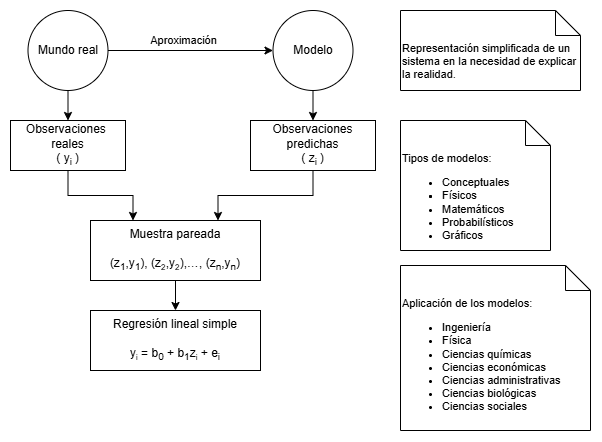
\includegraphics[width=0.7\linewidth]{recurso/regresion.png}
		\label{fig:valModel}
	\end{figure}
	
\end{frame}



\begin{frame}{Validación de un modelo con regresión lineal simple}

\begin{columns}
	% Columna para el texto (izquierda)
	\begin{column}{0.5\textwidth}
		\begin{exampleblock}{Exactitud y Precisión}
		\end{exampleblock}	
		\vspace{0.5cm}
		\begin{itemize}
			\item Exactitud: qué tan cerca están los valores reales de los valores predichos.
			\vspace{.3cm}
			\item Precisión: qué tan cerca están entre ellos los valores predichos por el modelo.
		\end{itemize}
	\end{column}
	
	% Columna para la figura (derecha)
	\begin{column}{0.5\textwidth}
		\centering
		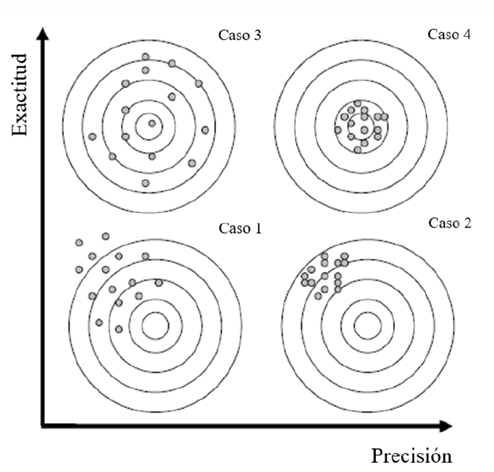
\includegraphics[width=\linewidth]{recurso/tadeshi_casos.png}
	\end{column}
\end{columns}
\end{frame}



\begin{frame}{Validación de un modelo con regresión lineal simple}
	
	\begin{exampleblock}{¿Cómo evalúa la Exactitud y Precisión?}
	\end{exampleblock}	
	
	Dada la muestra pareada $(z_{1}, y_{1}), (z_{2}, y_{2}) , \dots , (z_{n}, y_{n})$ se considera el modelo de regresión lineal:
	
	\begin{center}
		$y_{i}= \beta_{0} + \beta_{1}z_{i} + \epsilon_i$, donde $ 1 \leq i\leq n$.
	\end{center} 
	
	El modelo evaluado es exacto si $\mathbf{\beta_{0} = 0}$ y  $\mathbf{\beta_{1} = 1}$. Y es preciso si el coeficiente de determinación $R^2$ está cercano a 1.
	
	\vspace{0.3cm}
	
	Inconvenientes:
	\begin{itemize}
		\item Las pruebas estadísticas para evaluar la exactitud dependen del supuesto de normalidad y de varianza constante de los $\epsilon_i$.
		\item La precisión se mide de manera determinística. 
	\end{itemize}
\end{frame}



\begin{frame}{Trabajos realizados para evaluación de la exactitud y precisión}
	
	\begin{itemize}
		
				
		\item Balam, R. (2012). "Evaluación de la exactitud y precisión de un modelo con regresión lineal”. Tesis de Maestría, Facultad de Matemáticas, Universidad Autónoma de Yucatán.
		\vspace{0.3cm}
		
		 Para los casos: 
	\begin{itemize}
		\item[a)]	NVC se propuso una región de confianza con la F conjunta para evaluar la exactitud y un ICB BCa con residuales balanceados para la precisión.
		\vspace{.2cm}
	
		\item[b)] 		NNVC se emplearon ICB Percentil con sesgo corregido y un ICB BCa para evaluar la exactitud y la precisión respectivamente, ambos con los residuales balanceados.
		\vspace{.2cm}
		
		\item[c)] 		NVD y NNVD se emplearon ICB Percentil con sesgo corregido y un ICB BCa para evaluar la exactitud y la precisión respectivamente, ambos con las muestras pareadas balanceadas.
	\end{itemize}
		

	\end{itemize}
	
\end{frame}




\begin{frame}{Trabajos realizados para evaluación de la exactitud y precisión}
	
	\begin{itemize}
		\item  Zacarías, K. (2023). "Evaluación de la exactitud de un modelo cuando no se cumplen Los supuestos en la técnica de regresión lineal". Tesis de Maestría, Facultad
		de Matemáticas, Universidad Autónoma de Yucatán.
	\end{itemize}
	
	
	
	\begin{itemize}
		\item [a)] Se propone la construcción de una región de confianza para el vector ($\beta_0 , \beta_{1}$) con diferentes esquemas Bootstrap robustos. Si el punto (0,1) esta dentro de la región, el modelo es exacto, de lo contrario es inexacto.
		 
		\item[ b)] Se implementaron seis esquemas de remuestreo Bootstrap \textbf{para estimar la distribución de la estadística F conjunta} cuando no se cumplen los supuestos de normalidad y varianza constante: 
		
			\begin{itemize}
				\item[ i) ] El Bootstrap Robusto Simple.
				\item[ ii)] Los tres esquemas propuestos por Wu (1986).
				\item[ iii)] Y los dos esquemas propuestos por Lui (1988).
			\end{itemize}
		
		\item[ c)] Se propuso un estimador para el cuantil de la distribución F conjunta estimada.
	\end{itemize}

	
\end{frame}



\begin{frame}{El coeficiente de determinación $R^2$}
	
	\begin{exampleblock}{¿Cómo evaluar la precisión?}
	\end{exampleblock}	


	\begin{center}
	{\Large $R^{2} = \frac{ \sum_{i=1}^{n} ( \hat{y}_{i} - \bar{y})^{2}} { \sum_{i=1}^{n} ( y_{i} - \bar{y})^{2}  }$ }  y  $ 0 \leq R^{2} \leq 1$,
	\end{center}
	
	\vspace{0.3cm}
	
	Inconvenientes:
	\begin{itemize}
		\item No se conoce su distribución.
		\item No se puede usar para hacer predicciones.
		\item En presencia de valores atípicos o agrupamientos (clustering) en los datos, $R^{2}$ puede ser engañoso, pues un valor grande podría ser el resultado de estos factores, en lugar de un ajuste verdadero.
	\end{itemize}

\end{frame}




\begin{frame}{¿Cómo evaluar la precisión?}
	
\begin{center}
		En este trabajo se propone un método que permite evaluar la precisión de un modelo con la técnica de regresión lineal; y se basa en implementar diversos esquemas de remuestreo y estimar la precisión, a través de intervalos de confianza Bootstrap (ICB) para el coeficiente de determinación $R^2$, del modelo de regresión entre los valores reales y predichos del modelo que se desea evaluar.\
\end{center}
	
\end{frame}





%%%%%%%%%%%%%%%%%%%%%%%%%%%%%%%%%%%
\section{Objetivos}

\begin{frame}{Objetivo General}
Determinar la precisión de un modelo con la técnica de regresión lineal por medio de intervalos de confianza basado en diferentes esquemas de remuestreo Bootstrap y medir sus eficiencias a través de un estudio de simulación.
\end{frame}


\begin{frame}{Objetivo Específicos}
\begin{enumerate}
	\item Desarrollar la metodología para medir la precisión de un modelo con la técnica de regresión lineal por medio de intervalos de confianza basado en diferentes esquemas de remuestreo Bootstrap.
	\item Determinar la precisión de un modelo cuando se cumplan los supuestos de normalidad y varianza constante.
	\item Determinar la precisión de un modelo cuando no se cumplan los supuestos de normalidad y/o varianza constante.
\end{enumerate}
\end{frame}


\begin{frame}{Objetivo Específicos}
 \begin{enumerate}
	\setcounter{enumi}{3}
	\item Diseñar e implementar un estudio de simulación para evaluar la eficiencia de la metodología propuesta.
	\item Simular modelos exactos-precisos (EP) y modelos exactos-imprecisos (EI) mediante la propuesta de Febles (2014) y Zacarias (2023); cuando se cumplan o no los supuestos de normalidad e igualdad de varianzas.
	\item Determinar la eficiencia de los esquemas Bootstrap propuestos para medir la precisión de un modelo.
\end{enumerate}
\end{frame}


%%%%%%%%%%%%%%%%%%%%%%%%%%%%%%%%%%%%%%%%%%%%%%%%%%%%%%%%%%%%%%

\section{Metodología}

\begin{frame}{La propuesta}
	
	\begin{figure}[ht!]
		\centering 
		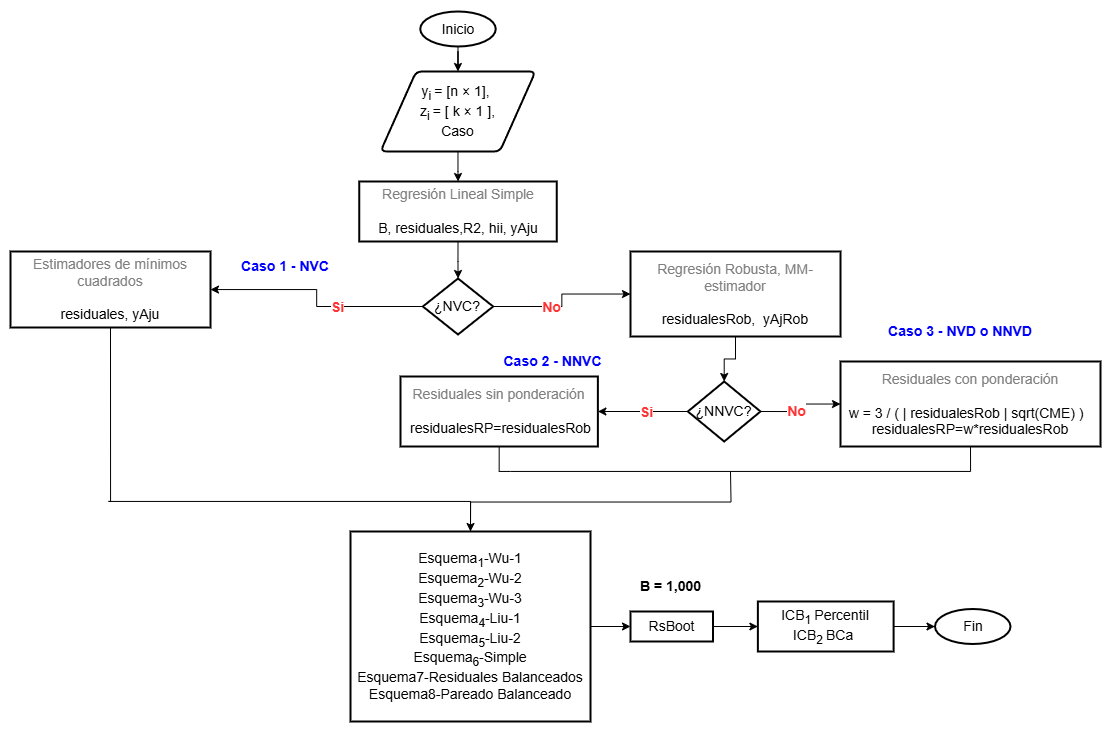
\includegraphics[width=0.75\linewidth]{recurso/metodoPresent_v8.png} 
		\label{fig:AlgDifEsqICBBoots}
	\end{figure}
	
\end{frame}








\begin{frame}{La propuesta}
	
	\begin{enumerate}
		\setcounter{enumi}{1}
		\item {\large \textbf{Esquemas de remuestreo Bootstrap para la estimación de $R^{2}$}.}\\
		
		Para los esquemas propuestos en Rana, es necesario generar una muestra Bootstrap $y^{*}_{i}$ dado por :
		
		\begin{center}
			{\large$y^{*}_{i} =z_{i}\hat{\beta}_{MM} + \frac{t^{*}_{i}\hat{e}^{WMM}_{i}}{\sqrt{1-h_{ii}}} $},
		\end{center}
		
		y ajustar la regresión simple:
		 \begin{center}
		 	$y^{*}_{i} = \beta_0^{*} + \beta_1^{*} z_i + \epsilon_i^{*} $,
		 \end{center}
		 
		 y obtener las nuevas $R^{2*}$ para estimar su distribución.
		
	\end{enumerate}
	
\end{frame}

\begin{frame}{La propuesta}
	
	\begin{itemize}
		\item \textbf{Wu 1}: $t^{*}_{i} \in N(0,1) , \; i= 1,\dots ,n$.
		
		\item \textbf{Wu 2}: Los $t^{*}_{i}$ corresponden a una muestra con reemplazo de los residuos normalizados.
		
		\item\textbf{ Wu 3}: El valor $t^{*}_{i}$ se obtiene mediante un remuestreo con reemplazo al vector de residuales transformados,
		
		\begin{center}
			{\large $R_{ai} = \frac{\hat{e}^{WMM}_{i} - Mediana(\hat{e}^{WMM}_{i})}{ NMAD(\hat{e}^{WMM}_{i})  }$} , $NMAD = \frac{1}{0.6745} Mediana\{ | \hat{e}^{WMM}_{i} - Mediana(\hat{e}^{WMM}_{i}) | \}$.
		\end{center}
		\vspace{0.2cm}
		
		\item \textbf{Liu 1}: $ t^{*}_{i} \in Gamma(4, 1/2),\; i= 1,\dots ,n$
	
		\item \textbf{Liu 2}: $t^{*}_{i} = H_{i}D_{i}- E(H_{i})E(D_{i}) $ donde \\
		
		$H_{i} \in N( 0.5\times \sqrt{17/6} + \sqrt{1/6} ,  0.5) = N(1.2498, 0.5) $ \\
		$D_{i} \in N( 0.5 \times \sqrt{17/6} - \sqrt{1/6} ,  0.5) = N(0.4334, 0.5), \; i= 1,\dots ,n$. Ambas independientes entre si.
		
	\end{itemize}
	
\end{frame}


\begin{frame}{La propuesta}
	
	Para los otros esquemas, para la muestra Bootstrap $y^{*}_{i}$ se obtiene remuestreando los residuales:
	
	\begin{center}
		{\large$ y^{*}_{i} = \hat{y}_{i} + e^{*}_{i}$},
	\end{center}
	
	y ajustar la regresión simple:
	\begin{center}
		$y^{*}_{i} = \beta_0^{*} + \beta_1^{*} z_i + \epsilon_i^{*} $,
	\end{center}
	
	y obtener las nuevas $R^{2*}$ para estimar su distribución.
	
	\begin{itemize}
		
		\item \textbf{Bootstrap Simple}:\\
		$e^{*}_{i}$ se obtienen de forma aleatoria con reemplazo de los residuales.
		
		\item \textbf{Bootstrap de Residuales Balanceados}:\\
		$e^{*}_{i}$ se obtiene de un conjunto aleatorio de residuales seleccionados de tal forma que cada uno aparece el mismo número de veces ($nB$).
		
	\end{itemize}
	
\end{frame}


\begin{frame}{La propuesta}
	
	\begin{itemize}
		\item \textbf{Bootstrap Pareado Balanceado}:\\
		
		Para la estimación de la distribución de la $R^{2*}$ se considera la muestra pareada $(y_i, z_i)$, y se remuestrea aleatoriamente $B$ veces con remplazo y de forma balanceada, para obtener las muestras \( \mathbf{y}_{1}^{*}, \mathbf{y}_{2}^{*}, \dots, \mathbf{y}_{B}^{*} \) y \( \mathbf{z}_{1}^{*}, \mathbf{z}_{2}^{*}, \dots, \mathbf{z}_{B}^{*} \) y ajustar una regresión simple entre los vectores \( \mathbf{y}^{*}_{i} \) y \( \mathbf{z}_{i}^{*} \), \( b = 1, 2, \dots, B \).
		
	
		
	\end{itemize}
	
\end{frame}




\begin{frame}{La propuesta}
	
	\begin{enumerate}
		\setcounter{enumi}{2}
		\item {\large \textbf{Cálculo del los intervalos de confianza para $R^2$}.}\\
		\vspace{.2cm}
	\end{enumerate}
	
	Intervalos de confianza Bootstrap Percentil (\textbf{ICB Percentil}) por esquema:
	
	\begin{enumerate}
		\item Se obtienen las muestras, $\hat{R}^{2*}_{1} , \hat{R}^{2*}_{2}, \dots,\hat{R}^{2*}_{B}$.
		
		\item Las $B$ muestras $\hat{R}^{2*}_{1}, \hat{R}^{2*}_{2},\dots, \hat{R}^{2*}_{B} $ se ordenan de manera ascendente, tal que $\hat{R}^{2*}_{1} \leq \hat{R}^{2*}_{2} \leq \dots \leq \hat{R}^{2*}_{B} $.
		
		\item Determinar los cuantiles $LI$ y $LS$, para el nivel de confianza del $(1-\alpha)$\% en la muestra Bootstrap ordenada, con $LI = \hat{R}^{2*}_{ ( \alpha/2 ) \: \times \: B} $ y $LS = \hat{R}^{2*}_{ (1 - \alpha/2) \: \times \: B} $.
		
		\item El intervalo de confianza esta dado por: $[LI_{per}, LS_{per}]$.
	\end{enumerate}
	 
\end{frame}



\begin{frame}{La propuesta}
	

	Intervalos de confianza Bootstrap BCa (\textbf{ICB BCa}) por esquema:

\begin{enumerate}
\item Obtener una estimación de la $\hat{R}^2$ a partir de los datos originales.

\item Se obtienen las muestras, $\hat{R}^{2*}_{1} , \hat{R}^{2*}_{2}, \dots,\hat{R}^{2*}_{B}$.

\item Se determina la proporción $p$ de las $\hat{R}^{2*}_{i}$ que son mayores o iguales a $\hat{R}^2$.

\item  Determinar $Z_{0} = Z_{p}$ donde $Z_{p}$ es el cuantil en la distribución normal estándar tal que $P(Z > Z_{p}) = p$.

\item  Obtener la constante de aceleración $a$ dada por:
\begin{center}
	\Large $ a = \frac{\sum_{i=1}^{n}  (\hat{R}^{2}_{-iprom}  - \hat{R}^{2}_{-i})^{3} }{ 6 \; (\; \sum_{i=1}^{n}  ( \hat{R}^{2}_{-iprom}  - \hat{R}^{2}_{-i})^{2} \; )^{3/2}} $ ,
\end{center}

donde: $\hat{R}^{2}_{-i}$ es la estimación con los datos originales quitando la $i$-ésima observación y {\normalsize $\hat{R}^{2}_{-iprom} = \frac{1}{n} \sum_{i=1}^{n}\hat{R}^{2}_{-i}$} .
\end{enumerate}
\end{frame}


\begin{frame}{La propuesta}
	
	
	Intervalos de confianza Bootstrap BCa (\textbf{ICB BCa}) por esquema (...continuación):
	
	\vspace{.3cm}
	
	\begin{enumerate}
		\setcounter{enumi}{5}
		
		\item Obtener {\large $Z_{L} = \frac{Z_{0} - Z_{\alpha/2}}{ 1- a ( Z_{0} - Z_{\alpha/2})} + Z_{0}  $}   y {\large $Z_{U} = \frac{Z_{0} + Z_{\alpha/2}}{ 1- a( Z_{0} + Z_{\alpha/2})} + Z_{0}  $}  donde: $Z_{\alpha /2}$ es el cuantil en la
		distribución normal estándar tal que $P(Z > Z_{\alpha / 2}) = \frac{\alpha}{2}$.
		
		
		\item Encontrar $LI = INVCDF( \Phi(Z_{L}))$ y $LS = INVCDF( \Phi(Z_{U}))$ donde $INVCDF$ es el cuantil en la muestra Bootstrap con probabilidad $ \Phi(Z_{L})$ y $ \Phi(Z_{U})$ respectivamente y $\Phi$ es la distribución acumulada de la normal estándar, siendo $P(\hat{R}^{2*} < LI) = \Phi(Z_{L})$ y$P(\hat{R}^{2*} < LS) = \Phi(Z_{U})$.
		
		\item El intervalo de confianza esta dado por: $[LI_{bca}, LS_{bca}]$.
	\end{enumerate}
\end{frame}










\begin{frame}{Diseño del estudio de simulación}
Para la simulación de los modelos se utilizaron los simuladores $\mathbf{ModNVC()}$, $\mathbf{ModNNVC()}$, $\mathbf{ModNNVD()}$ y $\mathbf{ModNVD()}$ (Febles, 2014; Zacarías, 2023). Se construyó la función $\mathbf{SimMod()}$ para la utilización de los simuladores.
\vspace{.3cm}

		
		\begin{table}[h!]
			\renewcommand{\arraystretch}{0.9} % Reduce el espacio vertical entre filas
			\scriptsize % Reduce el tamaño de la letra
			\begin{tabular}{|p{5cm}|p{5cm}|} % Ajusta los anchos de las columnas
				\hline
				\textbf{Exacto-Preciso (EP): 60,000 modelos} & \textbf{Exacto-Impreciso (EI): 60,000 modelos} \\ \hline
				
				
				\begin{itemize}
					\item $\beta_0 = 0$ y $\beta_1 = 1$
					\item $R^2$: aleatorio entre 0.8 y 0.99
					\item $n = 10, 15, 20, 25, 30$ y $35$
					\item Supuestos: NVC, NVD, NNVC, NNVD
					\item 500 modelos
					\item 5 replicas
				\end{itemize}
				 &
				  	
				 \begin{itemize}
				 	\item $\beta_0 = 0$ y $\beta_1 = 1$
				 	\item $R^2$: aleatorio entre 0.1 y 0.33
				 	\item $n = 10, 15, 20, 25, 30$ y $35$
				 	\item Supuestos: NVC, NVD, NNVC, NNVD
				 	\item 500 modelos
				 	\item 5 replicas
				 \end{itemize}
				 
				 \\ \hline
			\end{tabular}
		\end{table}
		
		
		En total se respaldaron 48 matrices que contienen los 120,000 modelos y 48 matrices que contienen las $R^2$ de origen correspondiente a cada modelo simulado.
		
\end{frame}




\begin{frame}{Eficiencias para los ICB }
	
	\begin{figure}[ht!]
		\centering 
		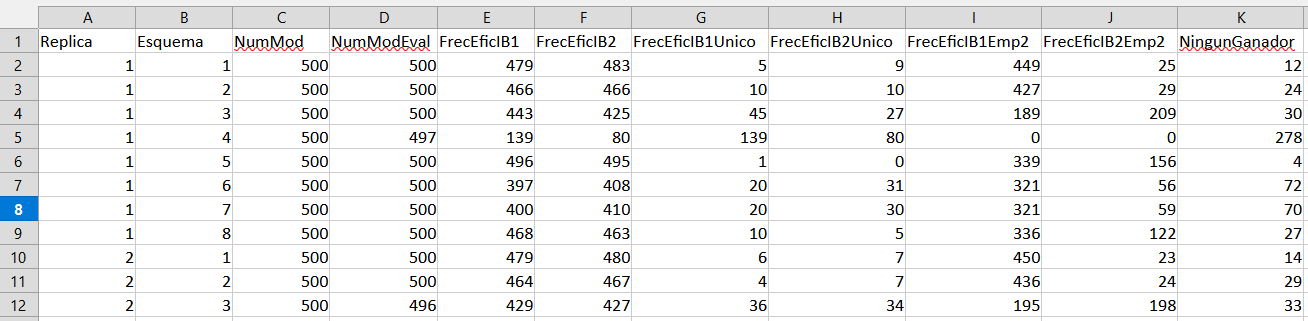
\includegraphics[width=0.9\linewidth]{recurso/tabla_eficiencia_intervalo.png} 
		\label{fig:tablaEficInt}
	\end{figure}
	
	
En total se construyeron 96 tablas para las eficiencias, de las cuales 48 fueron para modelos EP y 48 para modelos EI. Para resumir los resultados de las tablas se construyeron 8 nuevas tablas con las eficiencias promedio.
\end{frame}






\begin{frame}{Análisis estadísticos}
	Para cada supuesto (NVC, NNVC, NVD, NNVD) se utilizó ANOVA en un arreglo factorial de tres factores, donde: \\
	
	\begin{itemize}
		\item 	$y = $ Eficiencia del ICB (Percentil o BCa)
	
		\item 	$ \beta=$  Efecto del tamaño de la muestra (6 niveles).
	
		\item 	$ \tau=$ Efecto del esquema (8 niveles).
	
		\item 	$ \gamma=$ Efecto del tipo de modelo (2 niveles).
	\end{itemize}
	
	Para las comparaciones múltiples se utilizó Tukey al 5\%.
	\vspace{.3cm}
	
	
	En total se corrieron ocho ANOVAs, en cada comparación múltiple de Tukey se compararon 96 medias dando un total de 4,560 comparaciones de pares de medias.
\end{frame}



%%%%%%%%%%%%%%%%%%%%%%%%%%%%%%%%%%%%%%%%%%
\section{Resultados}
\begin{frame}{Comparación de la eficiencia del ICB Percentil para NVC}
		
		Cuando se tiene NVC y se utilizó el ICB Percentil para evaluar la precisión, se obtuvo interacción triple significativa ($TipoMod \times TM \times Esq: F=11.97, P<0.0001$). Con base en una eficiencia promedio de al menos 95\%, el mejor esquema
		resultó Liu2 sin importar el tamaño de muestra y tipo de modelo.
		\begin{figure} 
			\centering 
			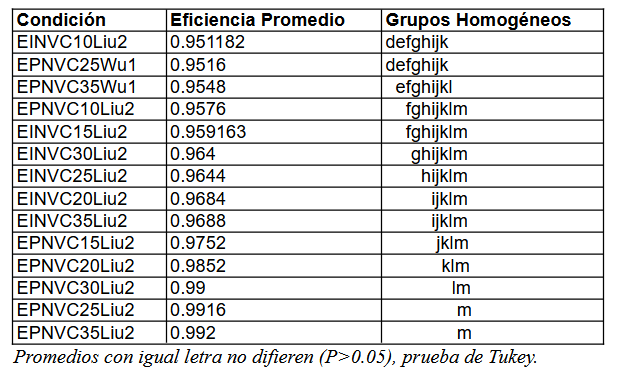
\includegraphics[width=0.60\linewidth]{recurso/CompEfic_PromICB_Perc_NVC.png} 
			\label{fig:CompEfic_PromICB_Perc_NVC}
		\end{figure}
	
\end{frame}



\begin{frame}{Comparación de la eficiencia del ICB BCa para NVC}
	
	Cuando se tiene NVC y se utilizó el ICB BCa para evaluar la precisión, se obtuvo interacción triple significativa ($TipoMod \times TM \times Esq: F=3.60, P<0.0001$).
	Con base en una eficiencia promedio de al menos 95\%, el mejor esquema resultó Liu2 sin importar el tamaño de la muestra, sin embargo, sólo identifica al tipo de modelo EP \textit{a priori} simulado.
	
	\begin{figure}[ht] 
		\centering 
		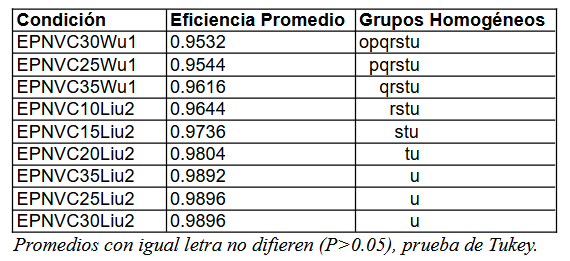
\includegraphics[width=0.72\linewidth]{recurso/CompEfic_PromICB_BCa_NVC.png} 
		\label{fig:CompEfic_PromICB_BCa_NVC}
	\end{figure}
	
\end{frame}




%%%NNVC

\begin{frame}{Comparación de las eficiencias de los ICB para NNVC}
  \begin{exampleblock}{Comparación con ICB Percentil:}
  		Con base en una eficiencia promedio de al menos 95\%, el mejor esquema resultó Liu2 sin importar el tamaño de muestra y tipo de modelo; con excepción del caso EINNVC10Liu2, sin embargo, su eficiencia promedio es 94.52\%.
  \end{exampleblock}
  
  \begin{exampleblock}{Comparación con ICB BCa:}
  	Con base en una eficiencia promedio de al menos 95\%, se obtuvo dos mejores esquemas Liu2 y Wu1 sin importar el tamaño de la muestra, sin embargo, ambos sólo identifican al tipo de modelo EP \textit{a priori} simulado.
  \end{exampleblock}
\end{frame}


%%%NVD

\begin{frame}{Comparación de las eficiencias de los ICB para NVD}
	\begin{exampleblock}{Comparación con ICB Percentil:}
		Con base en una eficiencia promedio de al menos 95\%, el mejor esquema resultó Liu2 sin importar el tamaño de muestra y tipo de modelo.
	\end{exampleblock}
	
	\begin{exampleblock}{Comparación con ICB BCa:}
		 Con base en una eficiencia promedio de al menos 95\%, el mejor esquema resultó Liu2 sin importar el tamaño de la muestra, sin embargo, sólo identifica al tipo de modelo EP \textit{a priori} simulado.
	\end{exampleblock}
\end{frame}


%%%NNVD

\begin{frame}{Comparación de las eficiencias de los ICB para NNVD}
	\begin{exampleblock}{Comparación con ICB Percentil:}
	Con al menos el 93.96\%, los dos mejores esquemas fueron Liu2 y ParBal para todos los TM con excepción de $n=35$ para Liu2 (92.72\%) y $n=10$ para ParBal (91.28\%). Ambos esquemas sólo identifican a los EI.
	\end{exampleblock}
	
	\begin{exampleblock}{Comparación con ICB BCa:}
	Con al menos el 88.80\%, con el esquema ParBal se obtuvo la mayor eficiencia promedio en todos los TM, también bajo el esquema Liu2 con excepción de $n=35$ (88.52\%) cuando el tipo de modelo es EP. El esquema ParBal identifica a los EI para $n= 25, 30, 35$ y las eficiencias no difieren estadísticamente con al menos 90.4\%.
	\vspace{.1cm}
	
	\textbf{En resumen:}
	Se determinó con al menos el 88.8\% que para el supuesto NNVD se utilice el ICB BCa con el esquema de remuestreo pareado balanceado; con la limitación de que para modelos EI con tamaños de muestra “pequeño” $n=10, 15, 20,$ no se obtuvo un buen desempeño.
	\end{exampleblock}
\end{frame}


%%%%%%%%%%%%%propuesta final
\begin{frame}{Propuesta final}
	\begin{figure}[ht] 
		\centering 
		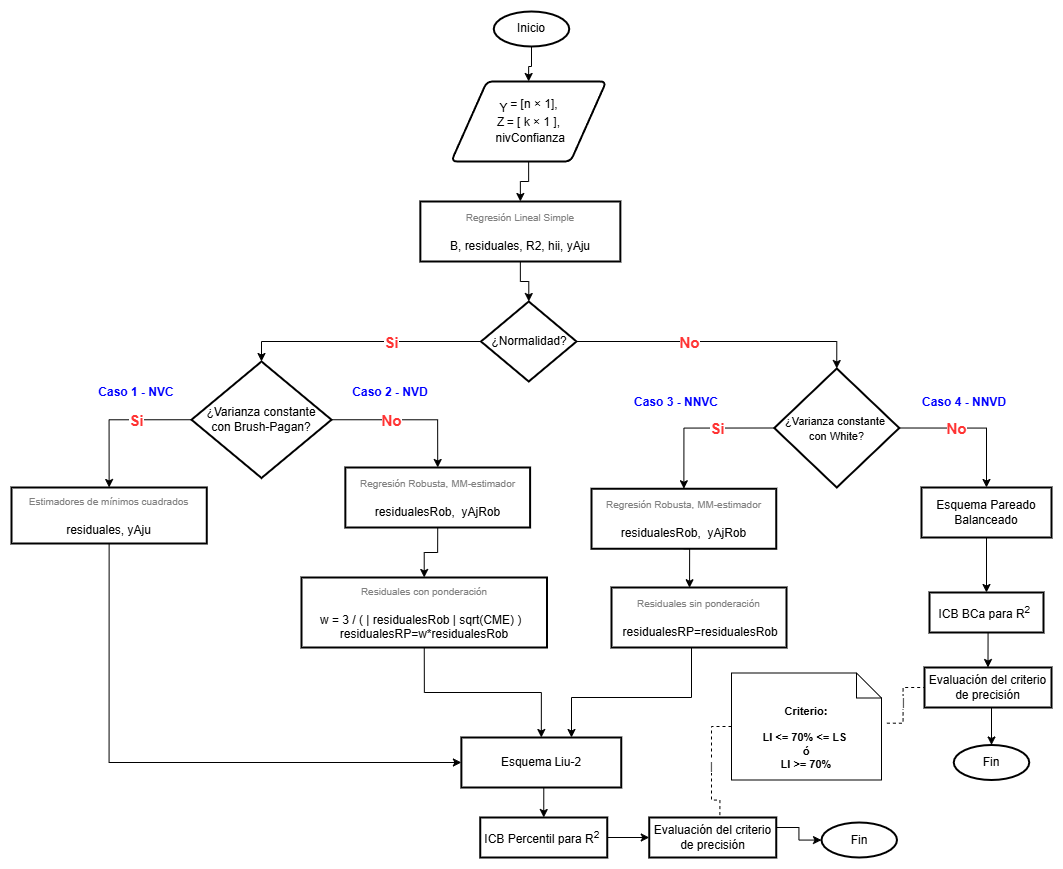
\includegraphics[width=0.62\linewidth]{recurso/finalPresent.png} 
		\label{fig:finalPropuesta}
	\end{figure}
\end{frame}


\begin{frame}{Aplicación de la propuesta final}
	\begin{exampleblock}{Caso NVC:}
		Para este caso se consideraron los datos experimentales de la ganancia diaria de peso (GDP) en ovinos; datos experimentales vs. modelo de simulación para estimar la ganancia diaria de peso (GDP) Osorio (2011). Estos datos se encuentran en el apéndice B de Balam (2012).
	\end{exampleblock}
\end{frame}


\begin{frame}{Aplicación de la propuesta final: Caso NVC}
	\begin{figure}[ht!]
		\centering 
		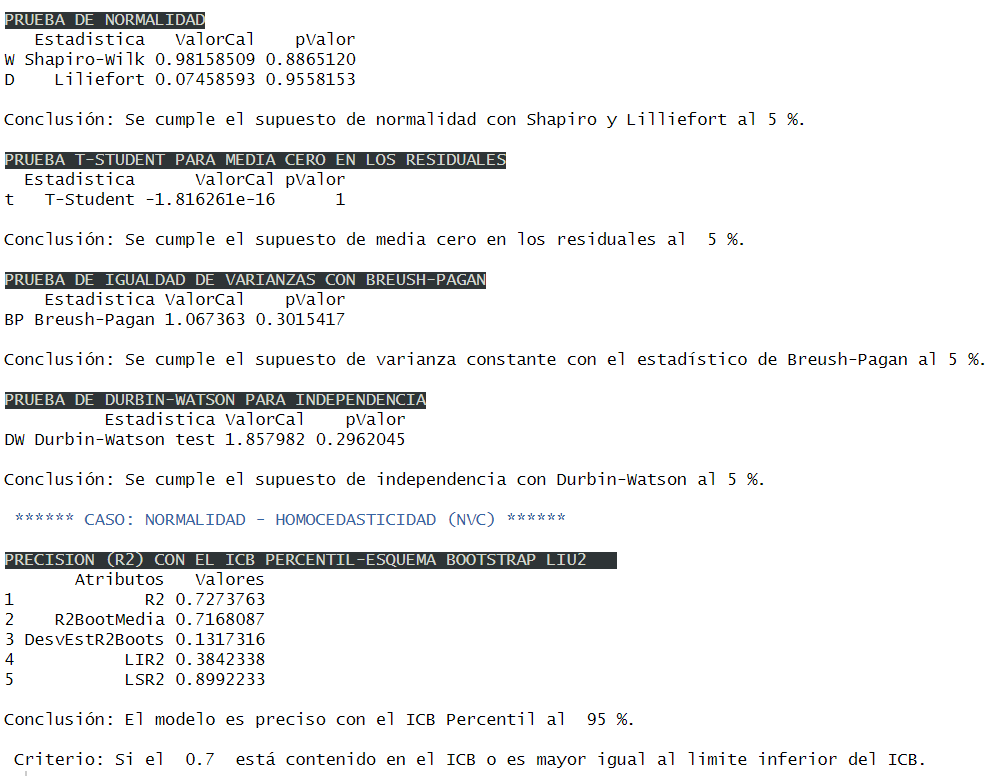
\includegraphics[width=0.65\linewidth]{recurso/Uso_NVC_PropuestaFinal.png} 
		\label{fig:final_NVC_resultados}
	\end{figure}
\end{frame}



\begin{frame}{Aplicación de la propuesta final}
	\begin{exampleblock}{Caso NNVD:}
		Se aplicó a los datos experimentales del volumen de una parcela en metros cúbicos a un diámetro superior $(n = 63)$ de 10cm y los simulados con el modelo PTAEDA Chung (1987), el cual es un modelo estocástico. Cada simulación con el modelo PTAEDA corresponde a la media de 10 corridas del modelo para cada parcela. En cada parcela se mide la edad, el indice de sitio y el número de arboles por hectárea. Estos datos se encuentran en el apéndice B de Balam (2012).
	\end{exampleblock}
\end{frame}


\begin{frame}{Aplicación de la propuesta final: Caso NNVD}
	\begin{figure}[ht!]
		\centering 
		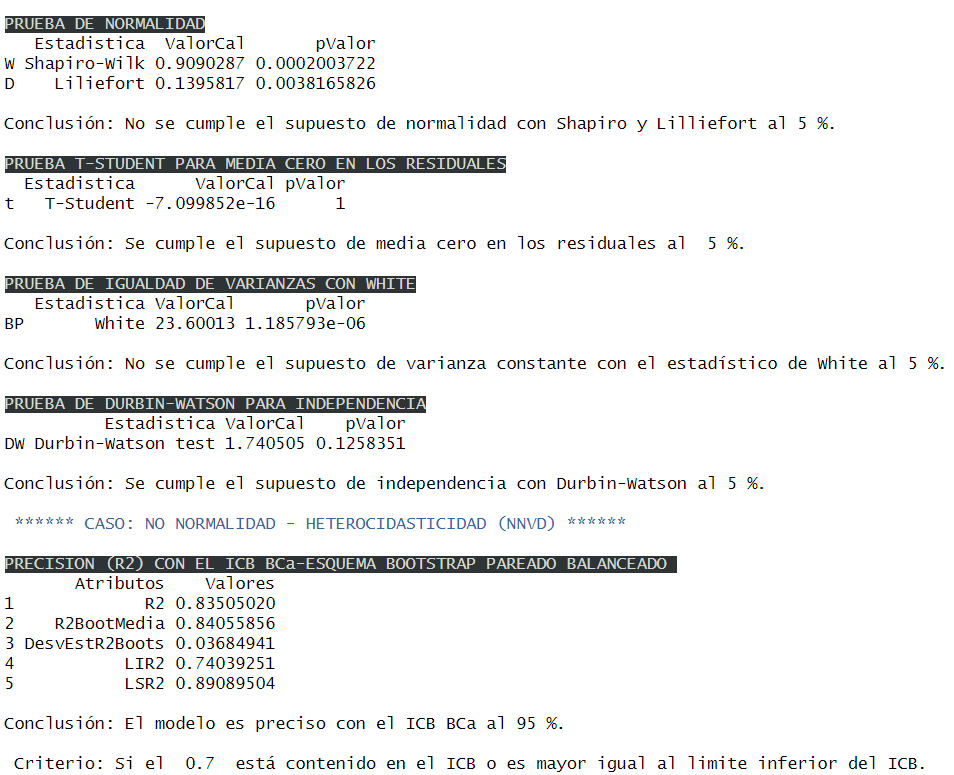
\includegraphics[width=0.62\linewidth]{recurso/Uso_NNVD_PropuestaFinal.png} 
		\label{fig:final_NNVD_resultados}
	\end{figure}
\end{frame}


\section{Conclusiones}
\begin{frame}
\begin{enumerate}
	\item 	Se propuso un método para evaluar la precisión de un modelo con la técnica de regresión lineal ; basado en ocho esquemas de remuestreo, dos tipos de modelo y seis tamaños de muestra; a través de dos ICB para el coeficiente de determinación $R^2$ y se consideraron los cuatro escenarios posibles (NVC, NNVC, NVD y NNVD) ante el cumplimiento o no normalidad y/o varianza constante.

	\item 	Se realizó un estudio de simulación para comparar las eficiencias de los intervalos de confianza para cada tipo de supuesto con respecto a los diferentes esquemas Bootstrap, tamaños de muestra y tipo de modelo.

	\item 	Análisis estadísticos: se determinó con al menos un 95\% que para los supuestos NVC, NNVC o NVD se utilice el ICB Percentil con el esquema de remuestreo Liu2 sin importar el tamaño de muestra. Y se determinó con al menos el 88.8\% que para el supuesto NNVD se utilice el ICB BCa con el esquema de remuestreo pareado balanceado.
\end{enumerate}
	

\end{frame}


\begin{frame}
	\begin{enumerate}
		\setcounter{enumi}{3}
		\item 	Propuesta final: para los supuestos NVC, NNVC o NVD se utilice el ICB Percentil con el esquema de remuestreo Liu2 (NVC: residuales de regresión lineal simple, NNVC: residuales robustos sin ponderar y NVD: residuales robustos ponderados) y para el supuesto NNVD se utilice el ICB BCa con el esquema de remuestreo Pareado Balanceado
		
		\item 	Se aplicó la propuesta final, para la ganancia diaria de peso en ovinos, el modelo resultó ser de tipo NVC y preciso, coincidiendo con Balam (2012), cabe señalar que usó ICB BCa con residuales balanceados y en este trabajo se usó ICB Percentil con el esquema de remuestreo Liu2. Para el volumen por parcela, el modelo resultó de tipo NNVD y preciso, coincidiendo con Balam (2012), tanto en la decisión como en el esquema e ICB que utilizó.
	\end{enumerate}
	
	
\end{frame}


\begin{frame}
	
	\begin{exampleblock}{Trabajos a futuro:}
		\begin{enumerate}
			\item Desarrollar una librería en el lenguaje R que contenga la propuesta de este trabajo para la evaluación de la precisión, junto con la propuesta desarrollada por \textcite{zacarias-2023} para la evaluación de la exactitud y de esta manera tener una herramienta integral para la evaluación de un modelo con la técnica de regresión lineal.
			
			\item Integrar la propuesta al Sistema de Validación de Modelos \parencite{mazun-2014}.
			
			
			\item Evaluar otros ICB que requieren cómputos más exhaustivos pero utilizando la programación en paralelo.
			
		\end{enumerate}
	\end{exampleblock}
	
\end{frame}







\section{Referencias}

\begin{frame}{Referencias}
	
    \printbibliography
\end{frame}


\begin{frame}
    \begin{center}
        {\Huge\calligra Muchas Gracias}
    \end{center}
\end{frame}

\end{document}